\newpage
\section{Theoretical Analysis}
\label{sec:analysis}

To make this analysis we used the following parameters values (of the circuit components that could be manipulated):


\begin{table}[h]
\centering
\begin{tabular}{ll}

Co & 1e-6 \\
Ci=Cb & 1e-3 \\
R1 & 80k \\
R2 & 20k  \\
RC & 1000 \\
RE & 100 
\end{tabular}
\end{table}

Hence the overall cost of the architecture is 1102.4 MU.

Considering the analyzed circuit, it is understood that the first stage is responsible for the amplication of the signal so that it is not degradated along the circuit. As such it is expected for it to have a high gain. 
Solving the OP problem with the help of Octave it is possible to obtaine $VCE=2.1578$

Regarding the gains plots between the first and 2 stage we can see that they do not differ alot, this is beliveble since AV2=-0.0348 db as we can see in the table, so it does not vary much the result.


\begin{figure}[h]
\centering
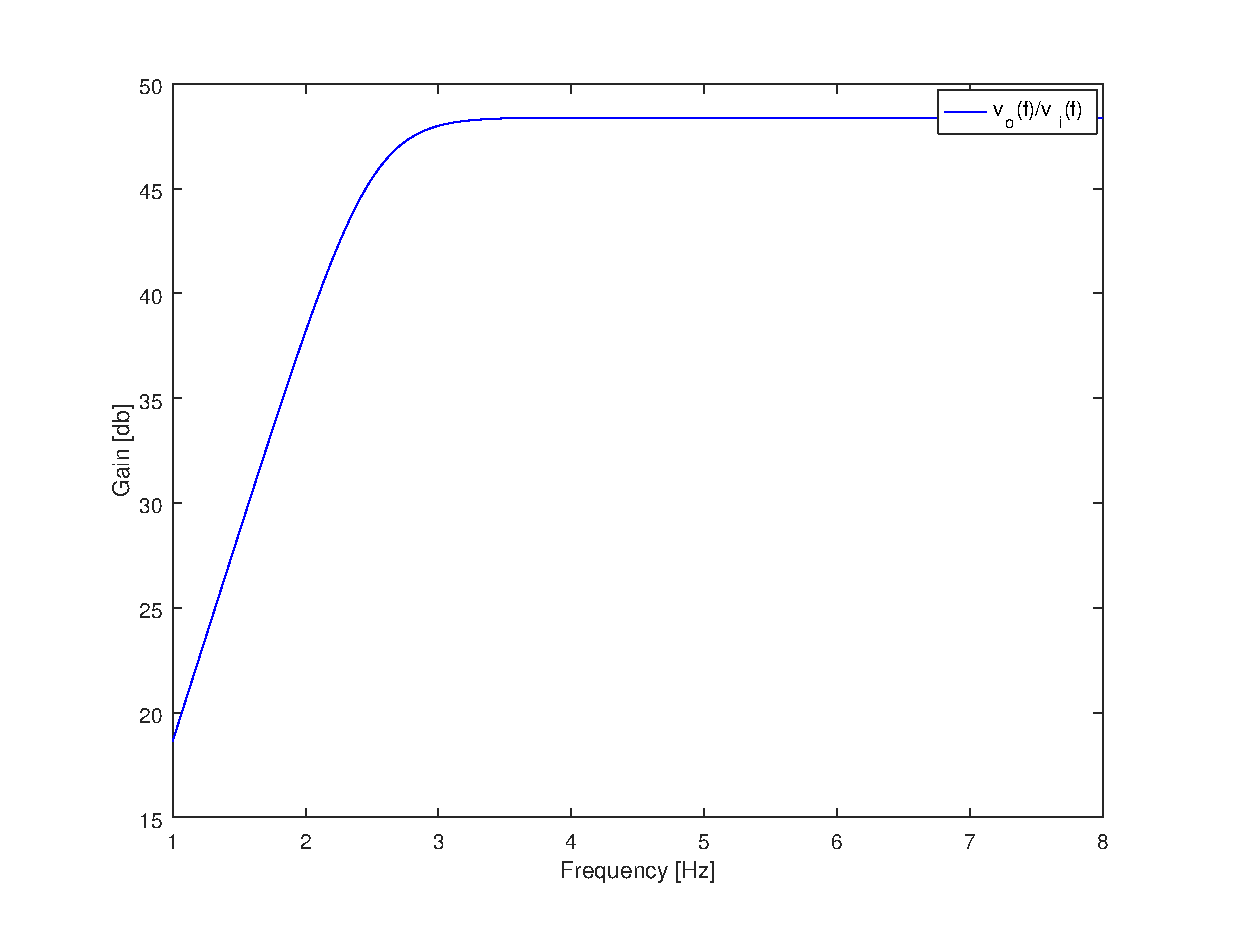
\includegraphics[width=0.6\linewidth]{Gain1.eps}
\caption{Gain in the first phase}
\label{plot:ganho1}
\end{figure}

\newpage

Nevertheless the inputs and outputs for this stages are present in the following table:

\begin{table}[h]
\centering
\begin{tabular}{ll}

AV1 & 48.39 \\
ZI1 & 484.43 \\
Z01 & 886.28 \\
AV2 & -0.0348  \\
ZI2 & 8598.9 \\
Z02 & 0.302 
\end{tabular}
\end{table}

\newpage

As we can see in the previous table, after the first stage the output impedance ($Z01$) increases. To contrariate that, it is added a new stage that decreases the output impedance. As a consequece we can connect this stages without a significant signal loss. Important to note that $AV2=0.996$, 
because it has a value near 1, this leads to small amplifications or attenuations
As such the final gain plot can be given by the following Figure.
\begin{figure}[h]
\centering
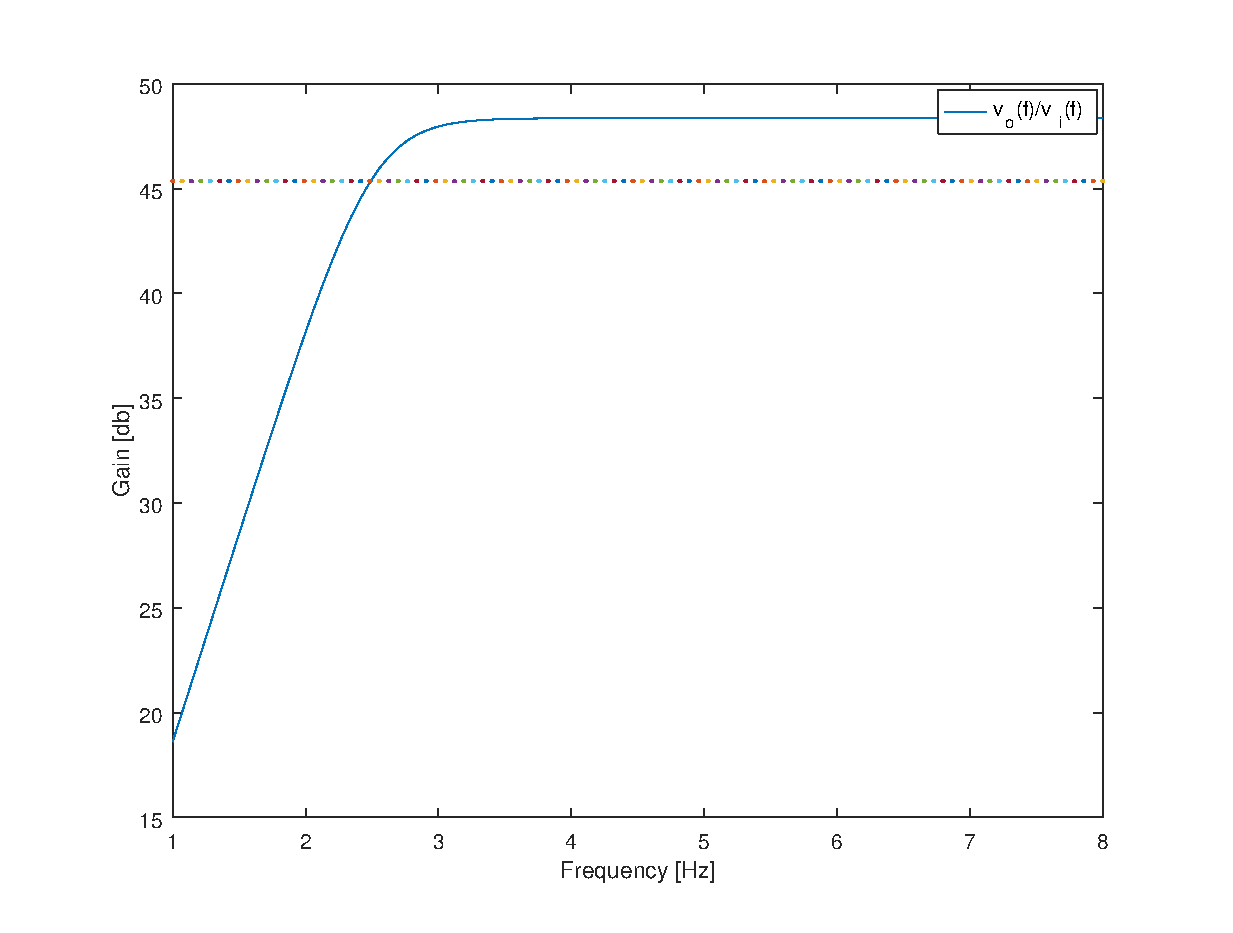
\includegraphics[width=0.6\linewidth]{GainFinal.eps}
\caption{Output Gain}
\label{plot:ganho2}
\end{figure}

Analyzing these plots we can see that they are high pass filter. Because it was expected a band pass an incorrect analsis of the circuit was most certainly made.